\scanpage{172}

gives

\deleted{\(\unsure{g_n\geq 3}\)}
\[
\underbrace{\underbrace{(2-2g_n)}_{\text{EP of }\widehat U_n}-3n}_{\text{EP}_{!}\text{ of }U_n}
=n^2\left(\underbrace{\underbrace{2}_{\text{EP of }\unsure{\widehat U_1}}-3}_{\text{EP of }U_1}\right)
\]

i.e.
\[
\inserted{2(g_n-1)=n^2-3n}
\qquad
\deleted{\unsure{2-2g_n=-n^2}}
\qquad \text{i.e.}
\]
\[
\text{(369)}\qquad g_n=\deleted{\unsure{2+}}1+\frac12 n(n-3)
\]

So we have
\[
\text{(370)}\qquad g_1=g_2=0,\quad g_3=1,\quad g_n>1\quad\text{if }n\geq\deleted{\unsure{3}}\inserted{4}.
\]

In any event, all the $U_n$ are anabelian, and even the $\widehat U_n$ for $n\geq4$.

If the \inserted{``\uline{anabelian}''} yoga developed in the first part of these notes is valid, the \deleted{\unsure{existence}} \deleted{(or the nonexistence) of} rational/$\mathbb Q$ points of a curve $U_n$ \deleted{\unsure{are explained by|are expressed by}} \inserted{correspond} to the \uline{splittings} of the extension of profinite groups

\noindent (371)
\diagram{\begin{tikzcd}[column sep=small]
1 \arrow[r] & \Pi_1(U_{n\overline{\mathbb Q}}) \arrow[r] &
\underset{\inserted{\substack{\unsure{\cap}\\\Pi_1(\unsure{U_1})\simeq\unsure{M_{0,3}^{!}}}}}{\Pi_1(U_n)} \arrow[r] & \Gamma_{\mathbb Q} \arrow[r] & 1
\end{tikzcd}}

which are distinct from the ``splittings at infinity'' (localized at the \inserted{3n} points at infinity of $U_n$\ldots), or again, the splittings such that \inserted{the \uline{centralizer} of} $(\Gamma_{\mathbb Q}^{+}=\operatorname{Ker}(\Gamma_{\mathbb Q}\xrightarrow{\chi}\widehat{\mathbb Z}^{*}))$ in $\Pi_1(U_n)$ is reduced to $\{1\}$. So -- if the ``theorem

\scanpage{173}
\mspage{734}

of Fermat'' is indeed valid (for $U_n$, say), it should be \unsure{reflected|reflected} in the nonexistence of such a splitting. Besides, if we \unsure{succeeded} in proving the nonexistence of splittings of (371) other than those ``coming from the points at infinity'', the theorem of Fermat would be proved for $U_n$, even without having established the ``anabelian yoga'' (a proof of which seems quite out of reach!). Now it is by no means excluded that a sufficiently thorough analysis of $M_{0,3}$ and $N_{1,1}$ in the present direction -- also involving finer and finer ``approximations'' of $\Pi_1(U_n)$ and of the extension structure (371), might eventually make it possible to prove the nonexistence of ``nontrivial'' splittings of (371), for all $n\geq3$. Each new refinement of the ``Lie approximations'' of $M_{0,3}$ should lead to a reexamination of the situation (371) and of the question of its splittings, with a view to a possible proof of the ``theorems of Fermat''.

\scanpage{174}

It is imperative to start from Lie approximations at least as fine as \unsure{those|that} of the present \S, which appears as the ``minima'' approximation in which one can express ``algebraically'' the tower of Fermat curves, \deleted{\unsure{where}} as we saw in 13\textsuperscript{o}), starting from $M_{0,3}\subset M_{0,3}^{\text{ét}}$.

Taking into account the operations of $\mathfrak S_3$ on $U_n$, the exact sequence (371) moreover embeds in a richer exact sequence

\noindent (372)
\diagram{\begin{tikzcd}[column sep=small]
1 \arrow[r] & \Pi_1(U_{n\overline{\mathbb Q}}) \arrow[r] &
\underset{\inserted{\substack{\cap\\\Pi_1(U_1,\mathfrak S_3)\simeq M_{0,3}}}}{\Pi_1(U_n,\mathfrak S_3)} \arrow[r] & \Gamma_{\mathbb Q}\times\mathfrak S_3 \arrow[r] & 1,
\end{tikzcd}}

and the calculations made in the present \S\ seem to suggest that this richer extension structure will play an important role.

From the point of view of the Lie approximation of $M_{0,3}$ developed in the present \S, it is appropriate to replace the extension structure (\unsure{372}) by a less fine quotient structure, by dividing by an invariant subgroup of $\Pi_1(U_n,\mathfrak S_3)$ contained in

\scanpage{175}
\mspage{735}

$\Pi_1(U_n,\overline{\mathbb Q})$, namely the intersection in $M_{0,3}$ of this group with $[\widehat\Pi_{0,3},\widehat\Pi_{0,3}]$. We find a commutative diagram

\noindent (373)
\diagram{\begin{tikzcd}[column sep=small,row sep=large]
1 \arrow[r] & \widehat M[n] \arrow[r] \arrow[d,"\unsure{1}"'] &
\begin{gathered}
\inserted{\overbrace{\Pi_1(U_n,\mathfrak S_3)^{\sim}}^{\unsure{\mathcal E_n}}}\\[-2pt]
\deleted{\unsure{\widetilde G_{\rho,\sigma}[n]}}
\end{gathered}
\arrow[r] \arrow[d,"\unsure{\text{epimorphism}}"] & \Gamma_{\mathbb Q}\times\mathfrak S_3 \arrow[r,no head] \arrow[d,"\chi\times\mathrm{id}"] & 1 \\
1 \arrow[r] & \widehat M[n] \arrow[r,no head] \arrow[d,hook] &
\widetilde G_{\rho,\sigma}[n] \arrow[r] \arrow[d,hook] & \widehat{\mathbb Z}^{*}\times\mathfrak S_3 \arrow[r,no head] \arrow[d,"\unsure{1}"] & 1 \\
1 \arrow[r] & \widehat M \arrow[r] & \widetilde G_{\rho,\sigma} \arrow[r] & \widehat{\mathbb Z}^{*}\times\mathfrak S_3 \arrow[r] & 1
\end{tikzcd}}

where the image of $\widehat M[n]\longrightarrow\widehat M$ is $n\widehat M$.

Here is \deleted{\illegible{1}} a way of constructing ``algebraically'' the diagrams (373) (for variable $n$) from the diagram

\noindent (374)
\diagram{\begin{tikzcd}[column sep=small,row sep=large]
1 \arrow[r] & \widehat M \arrow[r] \arrow[d,"\unsure{1}"'] &
\begin{gathered}
\overbrace{\Pi_1(U_1,\mathfrak S_3)^{\sim}}^{\mathcal E_1}\\[-2pt]
\Vert\\[-2pt]
(M_{0,3}/[\widehat\Pi_{0,3},\widehat\Pi_{0,3}])
\end{gathered}
\arrow[r] \arrow[d] & \Gamma_{\mathbb Q}\times\mathfrak S_3 \arrow[r,no head] \arrow[d,"\chi\times\mathrm{id}"] & 1 \\
1 \arrow[r,no head] & \widehat M \arrow[r] &
\begin{gathered}
\widetilde G_{\rho,\sigma}\\[-2pt]
\simeq(\widehat{\mathbb Z}^{*}\times\mathfrak S_3).\widehat M
\end{gathered}
\arrow[r] & \widehat{\mathbb Z}^{*}\times\mathfrak S_3 \arrow[r] & 1.
\end{tikzcd}}

We choose a \deleted{\unsure{which}} splitting of the first i.e. a splitting of the second (two such splittings are conjugate by a unique element of $\widehat M$\ldots).
\margin{We have seen that these splittings \inserted{\unsure{correspond|correspond}} \deleted{\unsure{being}} bijectively to those of the extension $\mathfrak S^{+\wedge}/\mu$ of $\mathfrak S_3$ by $\widehat M$, and we have defined a canonical one \deleted{\unsure{in}} $12^\circ)$.}
\deleted{\unsure{This is moreover}} \inserted{It can be inter}preted as a \inserted{geometric} point of $\unsure{U_\infty|U_n}$ above the

\scanpage{176}

base point $-\overline j$ of $U_{0,3\mathbb Q}\simeq U_{1\mathbb Q}$ -- it defines a geometric point of each of the $U_{n\mathbb Q}$ above $-\overline j$. In terms of this splitting of $\mathcal E_1$, allowing us to write
\[
\text{(375)}\qquad \mathcal E_1\simeq(\Gamma_{\mathbb Q}\times\mathfrak S_3).\widehat M
\qquad\text{($\frac12$ direct product)},
\]
the $\underset{\inserted{\substack{\unsure{\rotatebox{90}{$\simeq$}}\\\Pi_1(U_n,\unsure{\mathfrak S_n|\mathfrak S_3})/\ldots}}}{\mathcal E_n}\subset\mathcal E_1$ are identified with the semidirect products
\[
\text{(376)}\qquad \mathcal E_n=(\Gamma_{\mathbb Q}\times\mathfrak S_3).
\underbrace{(n\widehat M)}_{\overset{\text{definition}}{=}\widehat M[n]}
\]

(the interpretations are at the level of generalities of the proposition-lemma on page~$712'$ ff, and would deserve to appear in the \unsure{scholium|scholium}-proposition in question\ldots)

A \unsure{points|point} \inserted{$x_n$} \unsure{rational|rational}/$\mathbb Q$ of $U_n$ defines a splitting of the extension (of $\Gamma_{\mathbb Q}$ by $n\widehat M=\widehat M[n]$)
\[
\text{(377)}\qquad \underset{\inserted{\unsure{\varphi}}}{\mathcal E_n^{!}}\simeq\Gamma_{\mathbb Q}.(n\widehat M)
\qquad\text{($\frac12$ direct)}
\]
quotient of (371), knowledge of which
\scanpage{177}
\mspage{736}

modulo \deleted{\unsure{$n$}} $\widehat M[n]$-conjugation \uline{implies} that
of the corresponding splitting of $\mathcal E_1$, hence
implies knowledge of the corresponding point \inserted{$x_1$}
of $U_1(\mathbb Q)$ \deleted{\unsure{$x_1$}}, which means
that $x_n$ is known modulo the operation of
$\unsure{\gamma_n}=\mu_n(\mathbb Q)^{\{0,1,\infty\}}/\mu_n(\mathbb Q)$.
Now we have
\[
\begin{gathered}
\text{(378)}\qquad
\unsure{\gamma_n}\overset{\mathrm{dfn}}=
\mu_n(\mathbb Q)^{\{0,1,\infty\}}/\mu_n(\mathbb Q)=1\\
\text{if }n\text{ odd}
\end{gathered}
\]
for $\mu_n(\mathbb Q)=1$ if $n$ odd -- so in
this case $x_n$ is known when one knows
the corresponding splitting, and even
\unsure{only} its $\widehat M[n]$-conjugacy class.

This leads us to determine all these
possible $\widehat M[n]$-conjugacy classes of
such splittings, in order to examine (if it can be
done) which ones can reasonably
correspond to an $x_n\in U_n(\mathbb Q)$. These classes
correspond to the elements of
\[
\begin{aligned}
\text{(379)}\qquad
H^1(\Gamma_{\mathbb Q},n\widehat M)
&\simeq H^1(\Gamma_{\mathbb Q},\widehat M)
\simeq
\underbrace{H^1\unsure{(}\Gamma_{\mathbb Q},\widehat{\mathbb Z}(-1))}
_{\unsure{(\mathbb Q^*)^\wedge|(\mathbb Q^*]^\wedge}}
\otimes_{\mathbb Z}M\\
&\simeq G(\mathbb Q)^\wedge
\end{aligned}
\]

\scanpage{178}

where
\[
G\overset{\mathrm{dfn}}=
\unsure{\mathbb G_{m\,\mathbb Q}|G_{m\,\mathbb Q}}^{\{0,1,\infty\}}
/\unsure{\mathbb G_m|G_m}
\]
is the torus of dimension $2$ over $\mathbb Q$ in which
the $U_n$ are embedded. We see that
everything happens as if we were studying
simply the existence (!) and the cohomological
locating of the $\mathbb Q$-rational points of
$G$ itself -- without concerning ourselves
with the equation $x_0^n+x_1^n+x_\infty^n=1$ which defines
$U_n$. This shows plainly that
the approximation on which we are working
is much too coarse -- in fact,
in practice we \unsure{remain} in the
domain of a typically
``abelian'' analysis. It is clear that it is
necessary to pass to finer
approximations.

\scanpage{179}
\mspage{737}

\uline{52}\qquad
\uline{Schematic envelopes \unsure{of|of the} L-groups.}

$1^\circ)$ \uline{Notion of L-group}, \uline{of LT-group} (discrete case).

The notion of L-group is the natural
generalization of that of ``group with loops'',
which is called for if we want to be able to encompass
mixed fundamental groups of
orientable surfaces (of ``finite \unsure{character}'', i.e.
homeomorphic to an $X\setminus S$, $X$ a compact surface,
$S$ a finite subset) with a finite group of automorphisms.

We have seen that if $\Pi$ is a
group with loops (discrete), then every subgroup
of finite index $\Pi_0$ inherits a
loop structure, taking as
``loop subgroups'' of $\Pi_0$ the intersections
with $\Pi_0$ of the loop \unsure{subgroups} of $\Pi$. [N.B. we
assume that we are not in the cases
$(g,\nu)$ \deleted{\unsure{with}} with $g=0$, $\nu\in\{0,1\}$, where the loop structure
is \inserted{not} determined by the sole datum of a
family of conjugacy classes of \unsure{subgroups}
\deleted{\unsure{discrete}} $(\simeq\mathbb Z)$ -- the \inserted{only} case that would cause a problem here

\scanpage{180}

is the case $(0,1)$ \inserted{of $\Pi\simeq\mathbb Z$} -- in the case $(0,0)$, we have $\Pi=\{1\}$
and $\Pi_0=\Pi\ldots$ ]. Conversely, the loop
structure of $\Pi$ is recovered from
that of $\unsure{\Pi_{0*}|\Pi_0}$ (when it exists!), the
loop \unsure{subgroups} of $\Pi$ being the centralizers
in $\Pi$ of the \unsure{loop-subgroups} of $\Pi_0$.
\deleted{The exceptional case}

Let $\Pi$ be a discrete group,
\inserted{\deleted{finitely generated}}
\deleted{let} and
let $\mathcal L_0(\Pi)$ be the set of group-with-loops
structures on $\Pi$, of type $(g,\nu)$
\deleted{\unsure{with|$\ne$}}\inserted{\unsure{anabelian} i.e. $\ne$}
$(0,\unsure{0|1}),
\deleted{\unsure{(0,2)}}\inserted{(0,1)},
\deleted{\unsure{(1,0)}}\inserted{(1,0)}$.
For the subgroups \deleted{of} $\Pi_i$ \inserted{of $\Pi$} of finite index,
the $\mathcal L_0(\Pi_i)$ form an inductive system
\deleted{\unsure{with a map|with maps}}
of sets. \deleted{We set} If $\Pi_i$ is normal,
\[
\deleted{\mathcal L(\Pi)\qquad
\unsure{\mathcal L(\Pi_i)|\mathcal L_0(\Pi_i)}}
\]
we \deleted{\unsure{can}} \unsure{set|take}
\[
\deleted{\text{(1)}\qquad
\mathcal L(\Pi)=\varinjlim_i\mathcal L_0(\Pi_i)}
\]
\[
\begin{gathered}
\text{(1)}\qquad
\mathcal L_0^{\unsure{\natural|\sharp}}(\Pi_i)=
\text{set of loop structures}\\
\text{on }\Pi_i\text{ invariant under}\\
G_i=\Pi/\Pi_i.
\end{gathered}
\]

\deleted{We assume \unsure{that} $\Pi$ admits a finite
generating set, \unsure{hence a system}}
If there exists a $\Pi_{i_0}$ of finite index such that
$\mathcal L(\Pi_{\unsure{i|i_0}})\ne\varnothing$, then $\Pi_{i_0}$ hence also $\Pi$ admits
a finite generating set, and it follows
that the set of \inserted{\uline{normal}} subgroups of finite index
is cofinal in the set of subgroups
of finite index. We shall then set

\scanpage{181}
\mspage{738}

\[
\text{(2)}\qquad
\mathcal L(\Pi)=
\varinjlim_{\substack{\Pi_i\text{ normal}\\
\text{of finite index}\\
\text{in }\Pi}}
\mathcal L_0^{\unsure{\natural|\sharp}}(\Pi_i).
\]

\margin{N.B. If $\Pi_i$ is not normal in
$\Pi$, we can define
$\mathcal L_0^{\unsure{\natural|\sharp}}(\Pi_i)$ as the subset
of $\mathcal L(\Pi_i)$ formed by the loop
structures \inserted{$\lambda$} ``invariant under $\Pi$'', i.e. such that
for $\forall g\in\Pi$, we have that $\lambda$ (on $\Pi_i$) and
$\unsure{\mathrm{int}(g)|\mathrm{Int}(g)}\lambda$
(on $\unsure{\mathrm{int}(g)|\mathrm{Int}(g)}(\Pi_i)$) coincide in
$\Pi_i\cap\unsure{\mathrm{Int}(g)|\mathrm{int}(g)}(\Pi_i)$
(which is of finite index in $\Pi\ldots$)}

\deleted{We say that a}
the canonical morphisms ($\Pi_i$ normal of finite index
in $\Pi$)
\[
\text{(3)}\qquad
\diagram{\begin{tikzcd}
\mathcal L_0^{\unsure{\natural|\sharp}}(\Pi_i) \arrow[r] & \mathcal L(\Pi)
\end{tikzcd}}
\]
are injective. If $\lambda\in\mathcal L(\Pi)$, we say that
$\lambda$ is an \uline{L-structure}\unsure{.} on $\Pi$,
\inserted{$(\Pi,\lambda)$ is called an \uline{L-group},}
(and if
$\lambda\in\operatorname{Im}(\mathcal L_0^{\unsure{\natural|\sharp}}(\Pi_i)\to\mathcal L(\Pi))$),
we say that $\Pi_i$ is
a subgroup of definition of the L-group
$\Pi$ -- we regard it as a
group with loops via the unique $\lambda_i\in\mathcal L_0^{\unsure{\natural|\sharp}}(\Pi_i)$
giving rise to $\lambda$.

Let $\Pi$ be a discrete group, $\unsure{\Pi'_0|\Pi_0}$ a
subgroup of $\Pi$ of finite index. Then
we have a canonical homomorphism
for induction of L-structures
\[
\text{(4)}\qquad
\diagram{\begin{tikzcd}
\unsure{\mathcal L|\mathcal L_0}(\Pi) \arrow[r,hook] & \mathcal L(\Pi')
\end{tikzcd}}
\]
which is injective, and whose image consists
of the set of L-structures on $\Pi'$ that are
\scanpage{182}

``invariant under $\Pi$'' in an obvious sense.
In particular, if we have an \uline{extension}
of a finite group \inserted{$G$} by a
discrete group $\Pi_0$, then the $L$ structures on
$\Pi$ correspond to the $L$-structures
on $\Pi_0$ invariant under
$\Pi/\Pi_0\deleted{\unsure{\simeq G}}\inserted{\longrightarrow\unsure{\mathrm{Autext}}(\Pi_0)}$,
operating on the \unsure{set} of $L$-structures of $\Pi$
in an obvious way. [\uline{N.B.} $\Pi\mapsto\mathcal{L}(\Pi)$ is
a functor in the \uline{outer groups}
$\Pi$, with \uline{outer isomorphisms}
as arrows $\ldots$ ]

Standard example: let $X$ be an
anabelian surface ``of finite character'' \inserted{\unsure{0-connected}},
$G$ a finite group operating on $X$,
\[
\tag{\deleted{\unsure{4}}\inserted{5}}
\Pi=\Pi_1(X,G;\bullet)
\]
where $a$ is a base point of $X$, so
that we have an exact sequence
\[
\tag{6}
\diagram{\begin{tikzcd}[column sep=large,row sep=small]
1 \arrow[r,no head] & \Pi_0 \arrow[r] \arrow[d,equal] & \Pi \arrow[r] & G \arrow[r,no head] & 1 . \\
& \Pi_1(X,\bullet) & & &
\end{tikzcd}}
\]
We then have on $\Pi_0$ a loop structure
\scanpage{183}
\mspage{739}

invariant under the outer operations of $G$, hence
an $L$-structure on $\Pi$. It seems
that $\forall$ $L$-group is isomorphic to
a group obtained this way --- but this is
a result that seems
deep (essential\textsuperscript{ly} equivalent to that \unsure{of|of the}
\inserted{the existence} \inserted{of}
fixed points of finite subgroups of
Teichmüller groups $\ldots$), and which is
not completely understood. We should
\inserted{bring out} a general ``good statement'', linking the
$2$-category of $L$-groups, with that of
surfaces \inserted{$X$ of finite character, \deleted{\unsure{by some}}}
equipped \unsure{with a|with a} ``\unsure{signature}'' \inserted{$\underline{d}$} with
finite\deleted{\unsure{e}} support (with values in $\mathbb{N}^{*}$)
\inserted{punctured}, by associating to
such a surface its $\Pi_1(X,\underline{d},a)$,
relative to a point \deleted{base} $a\in X-\operatorname{supp}\underline{d}$.
Excluding a few singular cases \inserted{``trivial''}, we
should then find an $L$-group $\Pi$,
isomorphic to a $\Pi_1(X;G,a)$\unsure{,|;} with $G$
operating \uline{faithfully}, which \inserted{should} be expressed
\scanpage{184}

in terms of $\Pi$ by the fact that
the centralizer of $\forall$ subgroup
of finite index in $\Pi$ is reduced to $\{e\}$.
\unsure{This|This} should give a complete
\inserted{intrinsic} description, in topological terms, of the
$L$-groups having this additional property.
There would then still be
some work of \unsure{fitting together} to do,
in terms of certain extensions of
such $L$-groups by finite groups,
to \unsure{treat|find} the general case.
Moreover, we should make the connection
with the associated ``$L$-Galois topoi'',
paraphrasing the corresponding
developments on Galois topoi etc.
associated to groups with loops.
\scanpage{185}
\mspage{740}

It could be that the ``right'' general context
for defining and studying general
Teichmüller groups is that
of $L$-groups, rather than that of
groups with loops.

Taking for example the group \deleted{$\unsure{\mathfrak{M}|\mathfrak{S}}$}
\[
\tag{4}
\begin{aligned}
\deleted{\unsure{\mathfrak{M}_{0,3}^{+}|\mathfrak{S}_{0,3}^{+}}}\mathfrak{S}_{0,3}^{+}
&\simeq \mathrm{Sl}(2,\mathbb{Z})/\{\pm1\}\\
&\simeq \Pi_1(U_{0,3}(\mathbb{C}),\mathfrak{S}_3;-\overline{j}),
\end{aligned}
\]
this is equipped with an $L$-structure,
which can be defined in terms of
the unique conjugacy class of the
subgroup \inserted{$L_0$} generated by
$\varepsilon_0=\begin{pmatrix}1&-1\\0&1\end{pmatrix}$,
or of $L_1$ generated by
$\varepsilon_1=\begin{pmatrix}1&0\\1&1\end{pmatrix}$.
The $L$-group \inserted{(\uuline{discrete})} has the remarkable
property that every \inserted{$L$-}automorphism
\inserted{``direct'' (inducing the identity on the \unsure{orientation} module)}
of it is inner. It could
be that this property, added to
the property that the center is trivial (or
better, perhaps, that the centralizer
\scanpage{186}

of every subgroup of finite index is
reduced to $\{1\}$) characterizes $\mathfrak{S}_{0,3}^{+}$ up to
(nonunique) isomorphism.

N.B. To prove that every direct \inserted{$L$-}\unsure{automorphism|automorphism}
\inserted{$u$} of $\deleted{\unsure{\mathfrak M}}\mathfrak{S}_{0,3}^{+}$ is inner, the
essential point seems to me to be to prove
that $u$ preserves the subgroup
$\Pi_{0,3}$, kernel of
\[
\diagram{\begin{tikzcd}[column sep=large]
1 \arrow[r] & \Pi_{0,3} \arrow[r] & \deleted{\unsure{\mathfrak M}}\mathfrak{S}_{0,3}^{+} \arrow[r] & \mathfrak{S}_3 \arrow[r] & 1 .
\end{tikzcd}}
\]

In fact, every automorphism of
the group structure of $\mathfrak{S}_{0,3}^{+}$
(not necessarily an $L$-\unsure{automorphism|automorphism})
preserves the normal subgroup
$\Pi_{0,3}$. This follows from the

\uline{Lemma} Let \inserted{$\Pi\subset\mathfrak{S}_{0,3}^{+}$}
be a normal subgroup such
that $\mathfrak{S}_{0,3}^{+}/\Pi\simeq\mathfrak{S}_3$, then $\Pi=\Pi_{0,3}$.
More precisely, every surjective homomorphism
$p:\mathfrak{S}_{0,3}^{+}\deleted{\unsure{\Pi}}\longrightarrow\mathfrak{S}_3$ is conjugate to the canonical
homomorphism (hence its kernel is $\Pi_{0,3}$).

\uline{Proof} \deleted{Consider a surjective homomorphism}
\inserted{We use the presentation}
of $\mathfrak{S}_{0,3}^{+}$ by $\rho^3=\sigma^2=1$,
\scanpage{187}
\mspage{741}

which implies that a homomorphism $p$ from $\mathfrak S_{0,3}^{+}$ to another group, whose image is not of order $1,2$ or $3$ i.e. of order $\geq 4$, sends $\rho$ and $\sigma$ resp. to elements of order $3$ and of order $2$. So if the image is $\mathfrak S_3$, $\rho$ is sent to $\dot\rho$ or $\dot\rho^{-1}$ (we may suppose, conjugating if necessary \inserted{by $\dot\sigma_\infty$,} that it is $\dot\rho$) and $\sigma$ is sent to $\deleted{\unsure{\dot\sigma}}\;\dot\sigma_0,\dot\sigma_1$ or $\dot\sigma_\infty$ (we may suppose, conjugating by $\dot\rho$ or $\dot\rho^2$ if necessary, that it is $\dot\sigma_\infty$), and we win.

We may call the \uline{Teichmüller group} of an L-group $\Pi$, the group of its outer L-automorphisms --- or perhaps, better, the group of outer L-automorphisms of the subgroup $\Pi^+$ (of index $1$ or $2$) of $\Pi$, consisting of the $g\in\Pi$ such that the automorphism $\operatorname{int}(g)$ is direct. The property envisaged for $\mathfrak S_{0,3}^{+}$ is that its ``direct'' Teichmüller group is reduced to $1$. The property

\scanpage{188}

corresponding to this for the \inserted{L-}group $\mathfrak S_{0,3}\simeq\mathrm{Gl}(2,\mathbb Z)/\pm1$ is that every \deleted{group} \inserted{L-}automorphism of the subgroup $\mathfrak S_{0,3}^{+}$ is induced by a unique element of $\mathfrak S_{0,3}$. This property is perhaps characteristic of the \uline{discrete} L-group $\mathfrak S_{0,3}$.

\figure{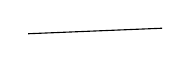
\begin{tikzpicture}
\draw (0,0) -- (1.7,0.07);
\end{tikzpicture}}

I feel like presenting in a slightly different form the notion of L-group\inserted{ $\Pi$,} in terms of the datum of a $\mathbb Z$-module $T$ free of rank $1$ (the $\mathbb Z$-module of orientations) and of a\deleted{\unsure{e}} \deleted{family} \inserted{finite set} $(k_i^{\unsure{\natural|\sharp}})_{i\in I}$ of \uline{germs} \uline{of homomorphisms} that are outer
\[
\begin{gathered}
k_i^{\unsure{\natural|\sharp}}:\quad \deleted{\unsure{\mathbb Z}}\inserted{T}\longrightarrow\Pi
\qquad (i\in I)\\
(\text{\uline{germ} of outer homomorphism})
\end{gathered}
\tag{5}
\]
,

where the notion of ``germ'' is relative to that of subgroups of finite index of $T$. \deleted{The axiom to put in is} \inserted{\unsure{For} such a datum,}

\scanpage{189}
\mspage{742}

and any subgroup \deleted{\unsure{to}} $\Pi_0$ of $\Pi$ of finite index, we find \inserted{for $\forall i$} a set of germs of outer homomorphisms
\[
T\longrightarrow\Pi_0
\]
induced by the actual homomorphisms \deleted{\unsure{outer}} $nT\longrightarrow\Pi$ of the class $k_i^{\unsure{\natural|\sharp}}$ --- we find a finite number of germs of outer homomorphisms $T\longrightarrow\Pi_0$ for fixed $i$, hence also for $i$ varying in $I$. This said, the only axiom of an L-structure, it is that we can find a subgroup $\Pi_0$ of finite index, such that the ``induced structure'' comes from a loop structure on $\Pi_0$.

We can generalize the notion of L-structure, taking inspiration from the preceding definition (for example), and dropping the requirement there that $\Pi_0$ be of finite index --- but while

\scanpage{190}

taking care on the other hand that $\Pi_0$ be \uline{normal}. We require that \deleted{the} for $\forall i\in I$, the germs of homomorphisms $k_i:\deleted{\unsure{n}}T\longrightarrow\Pi$ of the class $k_i^{\unsure{\natural|\sharp}}$ factor through $\Pi_0$ --- which gives a set of \inserted{germs of }outer homomorphisms from $T$ to $\Pi_0$ ---
\margin{N.B. it is not clear a priori that this set of germs of outer homomorphisms is finite}
and we require that this \deleted{set of} \inserted{structure in question} on $\Pi_0$ come \inserted{(for suitable $\Pi_0$)} from a loop structure on $\Pi_0$, \unsure{$\xi$|\&} obviously uniquely determined, once $\Pi_0$ has been chosen. As for $\Pi_0$, it is defined up to commensurability --- i.e. if $\Pi_0,\Pi'_0$ will do, then $\Pi_0\inserted{\cap}\Pi'_0$ is of finite index in $\Pi_0$ and $\Pi'_0$, and will do as well.

\deleted{Taking inspiration from the ``metabelian'' terminology,} I feel like (for want of a better suggestion) calling the groups $\Pi$ equipped with such a
